%
% coordinates.tex
%
% (c) 2019 Prof Dr Andreas Müller, Hochschule Rapperswil
%
\documentclass[tikz,11pt]{standalone}
%
% common.tex
%
% (c) 2020 Prof Dr Andreas Müller, Hochschule Rapperswil
%
\usepackage[T1]{fontenc}
\usepackage[utf8]{inputenc}
\usepackage{amsfonts}
\usepackage{amsmath}
\usepackage{amssymb}
\usepackage{times}
\usepackage{txfonts}
\usepackage{tikz}
\usetikzlibrary{arrows,intersections,math,calc,shapes.geometric,automata}
\usepackage{pgfplots}
\pgfplotsset{compat=1.16}
\usepackage{ifthen}


\begin{document}

\newboolean{showgrid}
\setboolean{showgrid}{false}
\def\breite{4}
\def\hoehe{4}

\begin{tikzpicture}[>=latex,thick]

% Povray Bild
\node at (0,0) {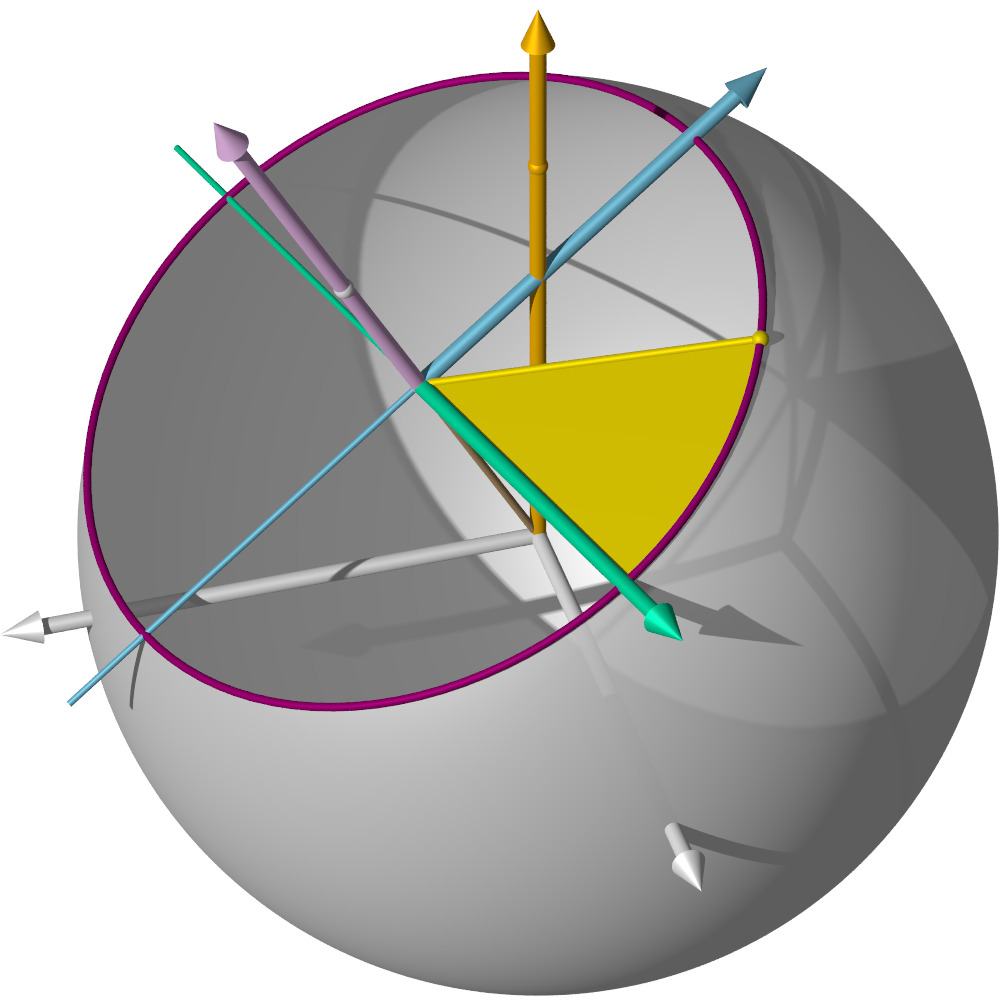
\includegraphics[width=8cm]{coordinates.jpg}};

% Gitter
\ifthenelse{\boolean{showgrid}}{
\draw[step=0.1,line width=0.1pt] (-\breite,-\hoehe) grid (\breite, \hoehe);
\draw[step=0.5,line width=0.4pt] (-\breite,-\hoehe) grid (\breite, \hoehe);
\draw                            (-\breite,-\hoehe) grid (\breite, \hoehe);
\fill (0,0) circle[radius=0.05];
}{}

\node at (1,0.5) {$\varphi$};
\node at (1.4,-1.1) [below] {$r_1$};
\node at (2.1,3.4) [right] {$r_2$};
\node at (-1.0,1.8) {$x$};
\node at (0.4,3.8) [right] {$n$};
\node at (-3.8,-1.4) {$x_1$};
\node at (1.5,-3.1) [left] {$x_2$};
\draw[<->] (0.16,-0.35) -- (-0.8,0.8);
\node at (-0.2,0.31) [below left] {$z$};

\end{tikzpicture}

\end{document}

